\documentclass[11pt,openany]{article}

\usepackage{mathtools, commath}
% Packages for formatting
\usepackage[margin=1in]{geometry}
\usepackage{fancyhdr}
\usepackage{enumerate}
\usepackage{graphicx}
\usepackage{kotex}
\usepackage{arydshln} % Include this package
\usepackage{bbding}
\usepackage{amsmath}
\usepackage{amsthm}
\usepackage[dvipsnames,table]{xcolor}
\usepackage{amssymb, amsfonts}
\usepackage{wasysym}
\usepackage{footnote}
\usepackage{tablefootnote}
\usepackage{arydshln} % Include this package
% Fonts
\usepackage[T1]{fontenc}
\usepackage[utf8]{inputenc}
\usepackage{newpxtext,newpxmath}
\usepackage{sectsty}

% Define colors
\definecolor{TealBlue1}{HTML}{0077c2}
\definecolor{TealBlue2}{HTML}{00a5e6}
\definecolor{TealBlue3}{HTML}{b3e0ff}
\definecolor{TealBlue4}{HTML}{00293c}
\definecolor{TealBlue5}{HTML}{e6f7ff}

\definecolor{thmcolor}{RGB}{231, 76, 60}
\definecolor{defcolor}{RGB}{52, 152, 219}
\definecolor{lemcolor}{RGB}{155, 89, 182}
\definecolor{corcolor}{RGB}{46, 204, 113}
\definecolor{procolor}{RGB}{241, 196, 15}

\usepackage{color,soul}
\usepackage{soul}
\newcommand{\mathcolorbox}[2]{\colorbox{#1}{$\displaystyle #2$}}
\usepackage{cancel}
\newcommand\crossout[3][black]{\renewcommand\CancelColor{\color{#1}}\cancelto{#2}{#3}}
\newcommand\ncrossout[2][black]{\renewcommand\CancelColor{\color{#1}}\cancel{#2}}

\usepackage{hyperref}
\usepackage{booktabs}

% Chapter formatting
\definecolor{titleTealBlue}{RGB}{0,53,128}
\usepackage{titlesec}
\titleformat{\section}
{\normalfont\sffamily\Large\bfseries\color{titleTealBlue!100!gray}}{\thesection}{1em}{}
\titleformat{\subsection}
{\normalfont\sffamily\large\bfseries\color{titleTealBlue!50!gray}}{\thesubsection}{1em}{}

%Tcolorbox
\usepackage[most]{tcolorbox}
\usepackage{multirow}
\usepackage{multicol}
\usepackage{blindtext}

\usepackage[linesnumbered,ruled]{algorithm2e}
\usepackage{algpseudocode}
\usepackage{setspace}
\SetKwComment{Comment}{/* }{ */}
\SetKwProg{Fn}{Function}{:}{end}
\SetKw{End}{end}
\SetKw{DownTo}{downto}

% Define a new environment for algorithms without line numbers
\newenvironment{algorithm2}[1][]{
	% Save the current state of the algorithm counter
	\newcounter{tempCounter}
	\setcounter{tempCounter}{\value{algocf}}
	% redefine the algorithm numbering (remove prefix)
	\renewcommand{\thealgocf}{}
	\begin{algorithm}
	}{
	\end{algorithm}
	% Restore the algorithm counter state
	\setcounter{algocf}{\value{tempCounter}}
}

\usepackage{adjustbox}
% Header and footer formatting
\pagestyle{fancy}
\fancyhead{}
\fancyhf{}
\rhead{\textcolor{TealBlue2}{\large\textbf{Linear Algebra \& Abstract Algebra}}}%\rule{3cm}{0.4pt}}
%\chead{\textcolor{TealBlue}{\large\it Think Globally, Act Locally}}
\lhead{\textcolor{TealBlue2}{\large\textbf{[Summer 2025] Mathematics Seminar}}}
% Define footer
%\newcommand{\footer}[1]{
%\begin{flushright}
%	\vspace{2em}
%	\includegraphics[width=2.5cm]{school_logo.jpg} \\
%	\vspace{1em}
%	\textcolor{TealBlue2}{\small\textbf{#1}}
%\end{flushright}
%}
%\rfoot{\large Department of Information Security, Cryptogrphy and Mathematics, Kookmin Uni.\includegraphics[height=1.5cm]{school_logo.jpg}}
\fancyfoot[L]{\large\it \textcolor{TealBlue}{\bfseries Think Globally, Act Locally}}
\fancyfoot[C]{-\thepage-}

\usepackage{tcolorbox}
\tcbset{colback=white, arc=5pt}

\definecolor{axiomcolor}{HTML}{a88bfa}
\definecolor{defcolor}{RGB}{52, 152, 219}
\definecolor{procolor}{RGB}{241, 196, 15}
\definecolor{thmcolor}{RGB}{231, 76, 60}
\definecolor{lemcolor}{RGB}{155, 89, 182}
\definecolor{corcolor}{RGB}{46, 204, 113}
\definecolor{execolor}{RGB}{90, 128, 127}

% Define a new command for the custom tcolorbox
\newcommand{\axiombox}[2][]{%
	\begin{tcolorbox}[colframe=axiomcolor, title={\color{white}\bfseries #1}]
		#2
	\end{tcolorbox}
}

\newcommand{\defbox}[2][]{%
	\begin{tcolorbox}[colframe=defcolor, title={\color{white}\bfseries #1}]
		#2
	\end{tcolorbox}
}

\newcommand{\lembox}[2][]{%
	\begin{tcolorbox}[colframe=lemcolor, title={\color{white}\bfseries #1}]
		#2
	\end{tcolorbox}
}

\newcommand{\probox}[2][]{%
	\begin{tcolorbox}[colframe=procolor, title={\color{white}\bfseries #1}]
		#2
	\end{tcolorbox}
}

\newcommand{\thmbox}[2][]{%
	\begin{tcolorbox}[colframe=thmcolor, title={\color{white}\bfseries #1}]
		#2
	\end{tcolorbox}
}

\newcommand{\corbox}[2][]{%
	\begin{tcolorbox}[colframe=corcolor, title={\color{white}\bfseries #1}]
		#2
	\end{tcolorbox}
}



\usepackage{amsthm}

% Define custom theorem styles
\newtheoremstyle{dotless} % Name of the style
{3pt} % Space above
{3pt} % Space below
{\itshape} % Body font
{} % Indent amount
{\bfseries} % Theorem head font
{} % Punctuation after theorem head
{2.5mm} % Space after theorem head
{} % Theorem head spec

\newtheoremstyle{definitionstyle} % Name of the style
{3pt} % Space above
{3pt} % Space below
{} % Body font
{} % Indent amount
{\bfseries} % Theorem head font
{.} % Punctuation after theorem head
{2.5mm} % Space after theorem head
{} % Theorem head spec

% Applying custom styles
\theoremstyle{dotless}
\newtheorem{theorem}{Theorem} % Theorem environment with section-wise numbering
\newtheorem{proposition}[theorem]{Proposition} % Theorem environment with section-wise numbering
\newtheorem{lemma}[theorem]{Lemma} % Lemma shares the counter with theorem
\newtheorem{corollary}[theorem]{Corollary} % Corollary shares the counter with theorem

\theoremstyle{definitionstyle}
\newtheorem*{observation}{\textcolor{Magenta}{Observation}}
\newtheorem{definition}{Definition} % Definition shares the counter with theorem
\newtheorem{example}{Example} % Example shares the counter with theorem
\newtheorem{exercise}{Exercise} % Example shares the counter with theorem
\newtheorem{remark}{Remark} % Remark shares the counter with theorem
\newtheorem*{note}{Note}

\newtheorem*{definition*}{Definition} % Definition shares the counter with theorem
\newtheorem*{example*}{Example} % Example shares the counter with theorem
\newtheorem*{exercise*}{\textcolor{violet}{Exercise}} % Example shares the counter with theorem
\newtheorem*{remark*}{Remark} % Remark shares the counter with theorem


\usepackage{tikz}
\usepackage{tikz-cd}
\usepackage{tikz-3dplot}
\usepackage{pgfplots}
\pgfplotsset{compat=newest} % Adjust to your version of pgfplots
\def\Circlearrowleft{\ensuremath{%
		\rotatebox[origin=c]{180}{$\circlearrowleft$}}}
\def\Circlearrowright{\ensuremath{%
		\rotatebox[origin=c]{180}{$\circlearrowright$}}}
\def\CircleArrowleft{\ensuremath{%
		\reflectbox{\rotatebox[origin=c]{180}{$\circlearrowleft$}}}}
\def\CircleArrowright{\ensuremath{%
		\reflectbox{\rotatebox[origin=c]{180}{$\circlearrowright$}}}}
\usetikzlibrary{
	3d, % For 3D drawing
	angles,
	arrows,
	arrows.meta,
	backgrounds,
	bending,
	calc,
	decorations.pathmorphing,
	decorations.pathreplacing,
	decorations.markings,
	fit,
	matrix,
	patterns,
	patterns.meta,
	positioning,
	quotes,
	shadows,
	shapes,
	shapes.geometric,
	tikzmark
}
\tikzset{
	% single mid‐path arrow
	mid arrow/.style={
		decoration={
			markings,
			mark=at position 0.5 with {\arrow{Stealth[scale=1.2]}}
		},
		postaction={decorate},
	},
	% style for field arrows
	field arrow/.style={
		-{Stealth[scale=1.0]},
		thick,
		blue!70!black,
	},
}
\newcommand{\ie}{\textnormal{i.e.}}
\newcommand{\rsa}{\mathsf{RSA}}
\newcommand{\rsacrt}{\mathsf{RSA}\textendash\mathsf{CRT}}
\newcommand{\inv}[1]{#1^{-1}}

%New Command
%\newcommand{\set}[1]{\left\{#1\right\}}
\newcommand{\N}{\mathbb{N}}
\newcommand{\Z}{\mathbb{Z}}
\newcommand{\Q}{\mathbb{Q}}
\newcommand{\R}{\mathbb{R}}
\newcommand{\cR}{\mathcal{R}}
\newcommand{\C}{\mathbb{C}}
\newcommand{\F}{\mathbb{F}}
\newcommand{\nbhd}{\mathcal{N}}
\newcommand{\Log}{\operatorname{Log}}
\newcommand{\Arg}{\operatorname{Arg}}
\newcommand{\pv}{\operatorname{P.V.}}

\newcommand{\of}[1]{\left( #1 \right)} 
%\newcommand{\abs}[1]{\left\lvert #1 \right\rvert}
%\newcommand{\norm}[1]{\left\| #1 \right\|}

\newcommand{\sol}{\textcolor{magenta}{\bf Sol}}
\newcommand{\conjugate}[1]{\overline{#1}}

\newcommand{\res}{\operatorname{res}}
\DeclareMathOperator*{\Res}{\operatorname{Res}}

%\renewcommand{\Re}{\operatorname{Re}}
%\renewcommand{\Im}{\operatorname{Im}}

\newcommand{\cyclic}[1]{\langle #1 \rangle}
\newcommand{\uniform}{\overset{\$}{\leftarrow}}
\newcommand{\xmark}{\textcolor{red}{\XSolidBrush}}
\newcommand{\vmark}{\textcolor{green!75!black}{\CheckmarkBold}}

\newcommand{\gen}[1]{\langle #1 \rangle}
\newcommand{\Gen}[1]{\left\langle #1 \right\rangle}

\newcommand{\img}[1]{\text{Img}(#1)}
\newcommand{\Img}[1]{\text{Img}\left(#1\right)}
\newcommand{\preimg}[1]{\text{Img}^{-1}(#1)}
\newcommand{\Preimg}[1]{\text{Img}^{-1}\left(#1\right)}

\newcommand{\relation}{\mathrel{\mathcal{R}}}
\newcommand{\injection}{\rightarrowtail}
\newcommand{\surjection}{\twoheadrightarrow}
\newcommand{\id}{\textnormal{id}}

\newcommand{\eqclass}[1]{\left[#1\right]}

% Define custom colors for O and X
\newcommand{\yes}{\textcolor{blue}{\bf \fullmoon}}
\newcommand{\no}{\textcolor{red}{\bf \texttimes}}

\DeclarePairedDelimiter\ceil{\lceil}{\rceil}
\DeclarePairedDelimiter\floor{\lfloor}{\rfloor}
%\renewcommand{\floor}[#1]{\lfloor #1\rfloor}
%\newcommand{\Floor}[#1]{\left\lfloor #1\right\rfloor}
%\newcommand{\ceil}[#1]{\lceil #1\rceil}
%\newcommand{\Ceil}[#1]{\left\lceil #1\right\rceil}

\newcommand{\topology}{\mathscr{T}}
\newcommand{\sequence}[1]{\langle #1\rangle}
\renewcommand{\vec}[1]{\mathbf{#1}}
\setstretch{1.25}
\begin{document}
	\pagenumbering{arabic}
	\begin{center}
		\huge\textbf{Linear Algebra I}\\
		\Large-- Proof for Existence of Basis --\\
		\vspace{0.5em}
		\large{Ji, Yong-hyeon}\\
		%	\large{\ttfamily \url{https://github.com/Hacker-Code-J}}\\
		\vspace{0.5em}
		\normalsize{\today}\\
	\end{center}
	
	\noindent 
%	We cover the following topics in this note.
%	\begin{itemize}
%		\item[] \textbf{Part I}
%		\item Linear Combination, Spanning Set
%		\item Linearly Independent and Dependent
%		\item Basis
%		\item[] \textbf{Part II}
%		\item Partial Order; POSET
%		\item Total Order (Linear Order); TOSET
%		\item Maximal, Minimal, Hasse Diagram
%		\item[] \textbf{Part III}
%		\item Chain, Zorn's Lemma
%		\item Basis Theorem (Existence of Basis)
%		\item Invariance of Basis Cardinality; Dimension of Vector Space
%	\end{itemize}
%	\hrule\vspace{12pt}

%\newpage
\axiombox[Zorn's Lemma]{\begin{axiom*}
		Let $(P,\preceq)$ be a nonempty partially ordered set with property that every chain $C\subseteq P$ has an upper bound in $P$; that is, for every chain $C\subseteq P$, \[
		\exists u\in P\quad \text{such that}\quad \forall c\in C,\quad c\preceq u.
		\] Then $P$ contains at least one maximal element; that is, \[
		\exists m\in P\quad\text{such that}\quad\forall a\in P,\quad (m\preceq a)\implies(m=a).
		\]
\end{axiom*}}
%\begin{proof}
%	See \hyperlink{zorn}{Proof of Zorn's Lemma}.
%\end{proof}

%\vfill
\begin{observation}[Existence of Basis] Let $\mathcal{L}:=\set{S\subseteq \R^3:S\ \text{is linearly independent}}$.
	\ \begin{center}
		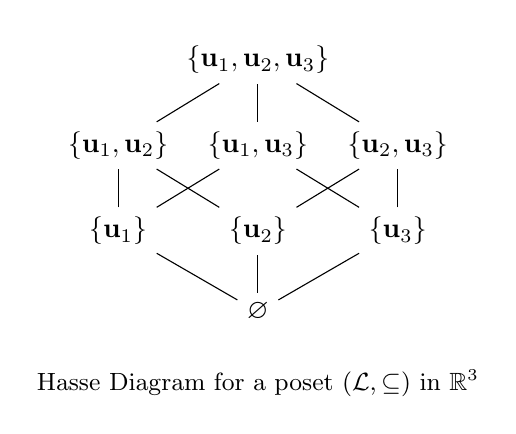
\begin{tikzpicture}
			\matrix (A) [matrix of nodes, row sep=.5cm]
			{ 
				&$\set{\vec{u}_1,\vec{u}_2,\vec{u}_3}$&\\
				$\set{\vec{u}_1,\vec{u}_2}$&$\set{\vec{u}_1,\vec{u}_3}$&$\set{\vec{u}_2,\vec{u}_3}$\\
				$\set{\vec{u}_1}$& $\set{\vec{u}_2}$ &$\set{\vec{u}_3}$\\
				& $\varnothing$ &\\
			};
			\draw (A-4-2)--(A-3-1);
			\draw (A-4-2)--(A-3-2);
			\draw (A-4-2)--(A-3-3);
			\draw (A-3-1)--(A-2-1);
			\draw (A-3-1)--(A-2-2);
			\draw (A-3-2)--(A-2-1);
			\draw (A-3-2)--(A-2-3);
			\draw (A-3-3)--(A-2-2);
			\draw (A-3-3)--(A-2-3);
			\draw (A-2-1)--(A-1-2);
			\draw (A-2-2)--(A-1-2);
			\draw (A-2-3)--(A-1-2);
			\node[draw=none, below=.25cm of A] {\small Hasse Diagram for a poset \((\mathcal{L},\subseteq)\) in \(\mathbb{R}^3\)};
		\end{tikzpicture}\hspace{40pt}
		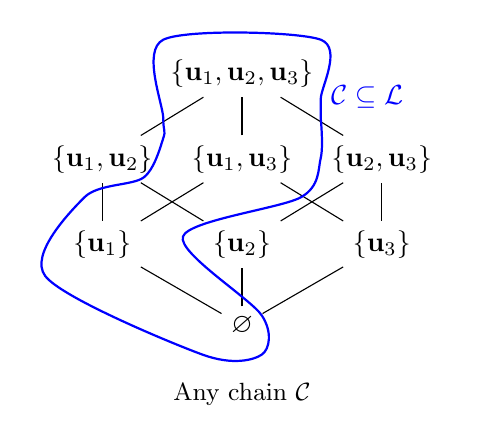
\begin{tikzpicture}
			\matrix (A) [matrix of nodes, row sep=.5cm]
			{ 
				&$\set{\vec{u}_1,\vec{u}_2,\vec{u}_3}$&\\
				$\set{\vec{u}_1,\vec{u}_2}$&$\set{\vec{u}_1,\vec{u}_3}$&$\set{\vec{u}_2,\vec{u}_3}$\\
				$\set{\vec{u}_1}$& $\set{\vec{u}_2}$ &$\set{\vec{u}_3}$\\
				& $\varnothing$ &\\
			};
			\draw (A-4-2)--(A-3-1);
			\draw (A-4-2)--(A-3-2);
			\draw (A-4-2)--(A-3-3);
			\draw (A-3-1)--(A-2-1);
			\draw (A-3-1)--(A-2-2);
			\draw (A-3-2)--(A-2-1);
			\draw (A-3-2)--(A-2-3);
			\draw (A-3-3)--(A-2-2);
			\draw (A-3-3)--(A-2-3);
			\draw (A-2-1)--(A-1-2);
			\draw (A-2-2)--(A-1-2);
			\draw (A-2-3)--(A-1-2);
			\node[draw=none, below=.25cm of A] {\small Any chain $\mathcal{C}$};
			
			\draw[color=blue,thick,smooth] plot coordinates {(1,1) (1,.5) (.75,0) (-.75,-.5) (.25, -1.5) (.25,-2) (-.5,-2) (-2.5,-1) (-2, 0) (-1.25,.25) (-1,.75) (-1, 1) (-1, 2) (1,2) (1,1.25) (1,1)} node[above right] {$\mathcal{C}\subseteq\mathcal{L}$};
		\end{tikzpicture}
	\end{center}
	\begin{center}
		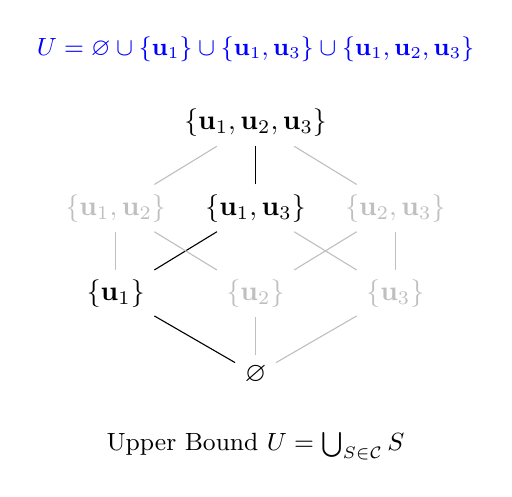
\begin{tikzpicture}
			\matrix (A) [matrix of nodes, row sep=.5cm]
			{ 
				&$\set{\vec{u}_1,\vec{u}_2,\vec{u}_3}$&\\
				\color{gray!50}$\set{\vec{u}_1,\vec{u}_2}$&$\set{\vec{u}_1,\vec{u}_3}$&\color{gray!50}$\set{\vec{u}_2,\vec{u}_3}$\\
				$\set{\vec{u}_1}$& \color{gray!50}$\set{\vec{u}_2}$ &\color{gray!50}$\set{\vec{u}_3}$\\
				& $\varnothing$ &\\
			};
			\draw (A-4-2)--(A-3-1);
			\draw[gray!50] (A-4-2)--(A-3-2);
			\draw[gray!50] (A-4-2)--(A-3-3);
			\draw[gray!50] (A-3-1)--(A-2-1);
			\draw (A-3-1)--(A-2-2);
			\draw[gray!50] (A-3-2)--(A-2-1);
			\draw[gray!50] (A-3-2)--(A-2-3);
			\draw[gray!50] (A-3-3)--(A-2-2);
			\draw[gray!50] (A-3-3)--(A-2-3);
			\draw[gray!50] (A-2-1)--(A-1-2);
			\draw (A-2-2)--(A-1-2);
			\draw[gray!50] (A-2-3)--(A-1-2);
			\node[draw=none, below=.25cm of A] {\small Upper Bound \(U=\bigcup_{S\in\mathcal{C}}S\)};
			\node[blue] at (0,2.5) {\small $U=\varnothing\cup\set{\vec{u}_1}\cup\set{\vec{u}_1,\vec{u}_3}\cup\set{\vec{u}_1,\vec{u}_2,\vec{u}_3}$};
		\end{tikzpicture}\hspace{40pt}
		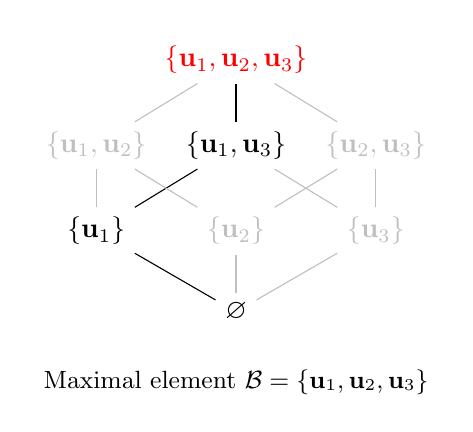
\begin{tikzpicture}
			\matrix (A) [matrix of nodes, row sep=.5cm]
			{ 
				&\color{red}$\set{\vec{u}_1,\vec{u}_2,\vec{u}_3}$&\\
				\color{gray!50}$\set{\vec{u}_1,\vec{u}_2}$&$\set{\vec{u}_1,\vec{u}_3}$&\color{gray!50}$\set{\vec{u}_2,\vec{u}_3}$\\
				$\set{\vec{u}_1}$& \color{gray!50}$\set{\vec{u}_2}$ &\color{gray!50}$\set{\vec{u}_3}$\\
				& $\varnothing$ &\\
			};
			\draw (A-4-2)--(A-3-1);
			\draw[gray!50] (A-4-2)--(A-3-2);
			\draw[gray!50] (A-4-2)--(A-3-3);
			\draw[gray!50] (A-3-1)--(A-2-1);
			\draw (A-3-1)--(A-2-2);
			\draw[gray!50] (A-3-2)--(A-2-1);
			\draw[gray!50] (A-3-2)--(A-2-3);
			\draw[gray!50] (A-3-3)--(A-2-2);
			\draw[gray!50] (A-3-3)--(A-2-3);
			\draw[gray!50] (A-2-1)--(A-1-2);
			\draw (A-2-2)--(A-1-2);
			\draw[gray!50] (A-2-3)--(A-1-2);
			\node[draw=none, below=.25cm of A] {\small Maximal element $\mathcal{B}=\set{\vec{u}_1,\vec{u}_2,\vec{u}_3}$};
		\end{tikzpicture}
	\end{center}	
\end{observation}

\newpage
\thmbox[$\star$ Basis Theorem $\star$]{\begin{theorem*}
		Every vector space $V$ over a field $F$ has a basis.
\end{theorem*}}
\begin{proof}
	\ \begin{flushleft}\color{red}
		\textbf{Key Idea}: ``By considering all linearly independent subsets of \(V\) and partially ordering them by inclusion, we use \underline{Zorn's Lemma} to guarantee a maximal linearly independent set exists.''
	\end{flushleft}
		\begin{enumerate}[Step 1]
				\item \textbf{Definition of Poset.}
				Define the set \[
				\mathcal{L}:=\set{S\subseteq V:\text{$S$ is linearly independent}}.
				\] with the partial order $\preceq$ on $\mathcal{L}$ by set inclusion: \[
				\forall S,T\in\mathcal{L},\quad S\preceq T\iff S\subseteq T.
				\] Since $\varnothing\in\mathcal{L}$, we have $\mathcal{L}\neq\varnothing$. Thus, $(\mathcal{L},\subseteq)$ forms a poset.
				\item \textbf{Chains and Upper Bounds.}
				Let $\mathcal{C}\subseteq\mathcal{L}$ be any chain, \ie, \[
				\forall S,T\in\mathcal{C},\quad S\subseteq T\ \text{or}\ T\subseteq S.
				\] Now, we need to find an upper bound $U\in\mathcal{L}$ of $\mathcal{C}$. Define \[
				U:=\bigcup_{S\in\mathcal{C}}S.
				\] Clearly, $U\subseteq V$. We claim that $U$ is linearly independent, \ie, $U\in\mathcal{L}$:
				\begin{enumerate}
						\item[] (\textit{Proof of $U\in\mathcal{L}$})\quad Let $n\in\N$ and suppose \[
						a_1\vec{u}_1+a_2\vec{u}_2+\cdots+a_n\vec{u}_n=0\quad\text{with}\ a_i\in F, \vec{u}_i\in U\ \text{for}\ i=1,2,\dots,n.
						\] Since $U=\bigcup_{S\in\mathcal{C}}S$, \[
						\vec{u}_i\in U\iff \exists S_i\in\mathcal{C}\ \text{such that}\ \vec{u}_i\in S_i
						\] for each $i\in\set{1,2,\dots,n}$. Since $\mathcal{C}$ is a chain (totally ordered by inclusion), the sets $S_1,S_2,\dots,S_n$ are comparable. Therefore, there exists at least one set $S^*\in\mathcal{C}$ such that \[
						(\forall i\in\set{1,2,\dots,n},\ \vec{u}_i\in S^*)\quad\ie,\quad\set{\vec{u}_1,\vec{u}_2,\dots,\vec{u}_n}\subseteq S^*.
						\] Since $S^*$ is an element of $\mathcal{C}$ (and $\mathcal{C}\subseteq\mathcal{L}$, where every element is linearly independent), the linear independence of $S^*$ implies that \[
						a_1=a_2=\cdots=a_n=0.
						\] Thus, $U$ is linearly independent, \ie, $U\in\mathcal{L}$.
					\end{enumerate}
				By definition of $U$, we know \[
				\forall S\in\mathcal{C},\ S\subseteq U,
				\] and so $U\in\mathcal{L}$ be an upper bound of $\mathcal{C}$.
				\item \textbf{Application of Zorn's Lemma.}
				
				Since every chain $\mathcal{C}$ in $\mathcal{L}$ has an upper bound $U\in\mathcal{L}$, Zorn's Lemma guarantees the existence of a maximal element $\mathcal{B}\in\mathcal{L}$ such that \[
				\forall S\in\mathcal{L},\ (\mathcal{B}\subseteq S)\implies (\mathcal{B}=S),\quad\ie,\quad\nexists S\in\mathcal{L}\ \text{with}\ \mathcal{B}\subseteq S.
				\]
				\item \textbf{$\mathcal{B}$ is a Basis of $V$.}
				
				We now show that $\mathcal{B}$ spans $V$, \ie, $\Span\mathcal{B}=V$. Assume, for contradiction, that \[
				\Span\mathcal{B}\neq V,\quad\ie,\quad\exists\vec{v}_0\in V\setminus\Span\mathcal{B}.
				\] Consider \[
				\mathcal{B}'=\mathcal{B}\cup\set{\vec{v}_0}.
				\] We NTS that $\mathcal{B}'$ is linearly independent. Suppose that for $n\in\N$, scalars $a_0,a_1,\cdots,a_n\in F$ and distinct vectors $\vec{v}_0,\vec{b}_1,\vec{b}_2,\cdots,\vec{b}_n\in\mathcal{B}'$, the followings holds: \[
				a_0\vec{v}_0+(a_1\vec{b}_1+a_2\vec{b}_2+\cdots+a_n\vec{b}_n)=0.
				\] \begin{enumerate}[(\text{Case} I)]
						\item If $a_0=0$, then \[
						a_1\vec{b}_1+a_2\vec{b}_2+\cdots+a_n\vec{b}_n=0
						\] and since $\mathcal{B}$ is linearly independent, $a_i=0$ for $i=1,2,\dots, n$.
						\item If $a_0\neq 0$, then \[
						\vec{v}_0=-\frac{1}{a_0}(a_1\vec{b}_1+a_2\vec{b}_2+\cdots+a_n\vec{b}_n)\in\Span\mathcal{B},
						\] which contradicts the assumption that $\vec{v}_0\notin\Span\mathcal{B}$.
					\end{enumerate}
				Thus, in all cases, \[
				a_0=a_1=\cdots=a_n=0.
				\] Hence, $\mathcal{B}'$ is linearly independent, \ie, $\mathcal{B}'\in\mathcal{L}$, and $\mathcal{B}\subseteq\mathcal{B}'$, contradicting the maximality of $\mathcal{B}$.
			\end{enumerate}
	
\end{proof}
\begin{remark*}
	This theorem and its proof is a classic demonstration of how abstract set-theoretic principles can yield concrete and essential results in linear algebra.
\end{remark*}
\end{document}
